% Proposal (3.5p)
\label{sec:proposal}


% Gena: Are you really following this approach???
%The rationale behind our approach is the following: an external agent (user or another system) creates a \emph{deployment request}, with goals that should be achieved in a given computing environment. A deployment agent, is responsible to handle that \emph{deployment request} autonomously. The deployment agent is capable of discover available resources in a computing environment it manages. That knowledge about the computing environment is the \emph{context} for the target deployment. The deployment agent is also capable of choosing artifacts from a repository that allows the satisfaction of the deployment request. The process of choosing the correct set of artifacts to allow the deployment request satisfaction is the \emph{deployment planning}.

% General discussion
Following the model proposed by Andersson et al.\cite{andersson_software_2013} for adaptive software development process, we divide our approach into \emph{offline} and \emph{online} activities. In this work, the \emph{offline} activities are conducted by software engineers and result in development and publishing of software components. The \emph{online} activities are autonomously executed in the target environment and result in the deployment of the system. Figure~\ref{fig:overview} presents an overview of the process.

\begin{figure*}[!htb]
  \centering
  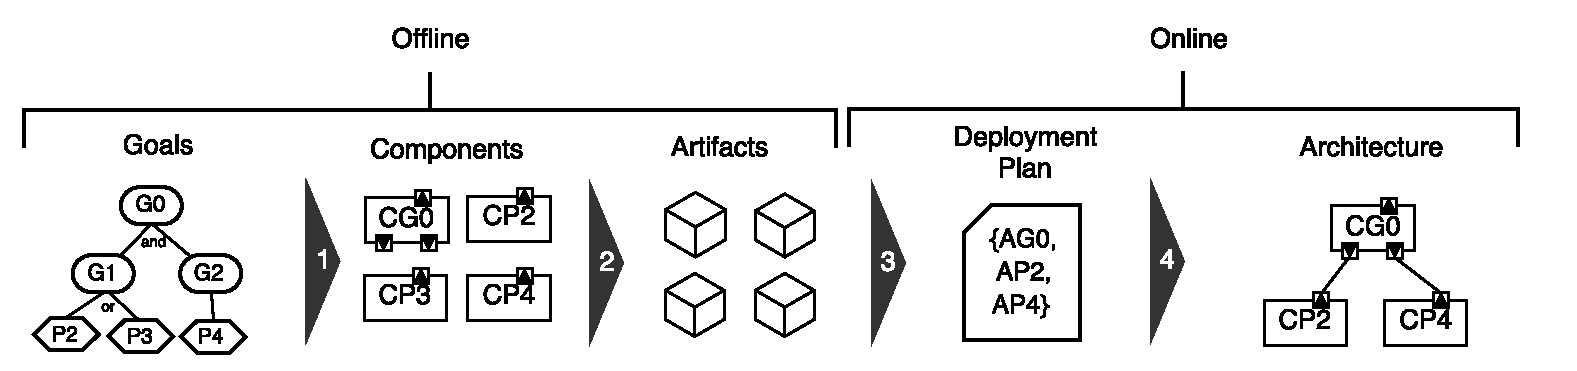
\includegraphics[width=1\linewidth]{transformations}
  \caption{Overview}
\label{fig:overview}
\end{figure*}

Figure~\ref{fig:overview} depics an overview of the process.
Activities: (1) component mapping; (2) packaging;
(3) deployment planning; (4) deployment execution.

In the offline part, occurs the design of the application. In the first step of our approach, components are mapped from the system CGM using patterns. In the second, these components are packaged into artifacts together with their metadata, which describes what goals the artifact provides, its context conditions and dependencies. These packaged artifacts are put in a repository.  Activities: (1) component mapping; \ref{} (2) packaging;\ref{}

In the online part of the approach, the Goalp deployment planning is executed in the target computing environment and autonomously finds a deployment plan.
The deployment planning is responsible for looking into the repository of artifacts and based on context information and goals, find a set of artifacts that should be deployed to the target computing environment in order to make the goals achievable.(3) deployment planning; (4) deployment execution.\ref{}



\section{Offline}

Previously, goal-driven  approaches were proposed for introducing variability at requirements, context modeling, software behavior, and software architecture\cite{angelopoulos_capturing_2015}\cite{yu_goals_2008}.
In our methodology, we propose a systematic approach to support deployment variability, from requirements to deployment.
Deployment variability is important since not taking into account the heterogeneity of a computing environment may lead to unnecessary or even unsuited deployment of components.
Such scenario would bring a negative impact to software performance, or in some cases represent inconsistent deployment of functionalities on the target device.

When developing a monolithic software, we implement in the same codebase all functionalities, then all code is built and deployed together.
In the Filling Station Advisor example, if implementing it as a monolithic software, the logic to get the vehicle position using GPS or antenna triangulation would stay in the same codebase and would be deployed altogether in the target environment, even when it does not have antenna triangulation capability.


In order to better cope with heterogeneity in the computing environment, we should minimize the coupling between parts of the code that have dependencies on specific resources in the environment.
By encapsulating dependencies of specific resources into components, it is possible to create variability at architecture level. By packaging the components into different artifacts, it is possible to maintain such variability at deployment level. Such variability is useful as it allows the deployment of components only to environment that have the required resources.

Regarding the Filling Station Advisor example, depicted in \ref{fig:goal_model_filling_station_advisor}, for goal \emph{G1}(Get Position), components can be implemented providing the actual position of the device by means of GPS or antenna triangulation. These components can be packaged into different artifacts that will only be deployed when the target environment has the appropriate resources.

\subsection{Resources as Context Information}
\label{context}

A systematic way of analyzing the capabilities of the computing environment is needed in order to support the resolution of variability at deployment-time. First, the available capabilities in the environment should be represented.

\begin{defn}[Resource]

  A resource provides a specific computing capability, it could be available in the computing environment and used in plans. A resource receives a label.

\end{defn}

Each resource relevant to the application receives a label.
Regarding the Filling Station Advisor, examples of relevant resources are \emph{GPS}, (labeled c1) and \emph{antenna triangulation} (labeled c2). Plans can require resources in order to be applicable, for example, \emph{P1: get position using GPS} requires the resource GPS to be available.

In order to reason about available resources in the target computing environment a context model is used. The context model reifies the computing environment.
In Goalp, the context of a target computing environment is a set of labels. The semantics is that if a label is present in the set, the resource is available in the target environment.

\begin{defn}[Context]

  A context Ctx := r1..rn, \{ r $\in$ Ctx | a resource labeled r is available in the computing environment\}
\end{defn}

In our example, the set
[c1, c5, c8] is an example of context, representing that GPS, connection to the Internet and voice synthesizing are resources available in the computing environment.

To evaluate if a plan is applicable in a given context we use \emph{context conditions}.

\begin{defn}[Context condition]
  A context condition cc:=TRUE iff cc:r, r $\in$ Ctx
\end{defn}

\emph{Conditions restrictions} represent restrictions to the applicability of a plan. Conditions restrictions are represented by labels and are evaluated against a context.
A context condition is satisfied if its associated label is present in the context. For example, in a scenario with context Ctx=[c1, c5], the context condition c1 holds while c2 do not.

Context conditions are used to solve variability. In Figure~\ref{fig:goal_model_filling_station_advisor}, the goal G1 has two alternatives to be achieved: by executing plan P1 or P2. The plan P1 is applicable if the context condition c1 holds, which is the case when GPS is available in the environment.

\subsection{Component Mapping}

\label{sec:goals_components}
Components are architectural units. In our proposal, components definitions are mapped from the CGM and them developed by the architect/developer. That activity is named component analysis. In our vision, components can \emph{provide} goals which means that they can be executed to \emph{fulfill} a goal at runtime.

The patterns present in table~\ref{table_cgm_to_components_patterns} are used, at the component analysis, to map components based on the CGM of the system. By mapping components we mean identifying which component should be developed in order to reflect the CGM of the system. By using the proposed patterns, the variability present in the CGM is kept at the architecture of the system. Theses patterns are an extension of Yu et al.\cite{yu_goals_2008} patterns for the Goals-Component view. We extended Yu et al.\cite{yu_goals_2008} patterns with contextual conditions.

\begin{table}[!htb]
\centering
\caption{Contextual Goal Model to components - patterns}
\label{table_cgm_to_components_patterns}
\bigskip
\begin{tabular}{|c| c p{5cm}|}
\hline
 %\textbf{ A } & \textbf{ B} & \textbf{C} \\ \hline
 And-Refinement &
 \raisebox{-\totalheight}{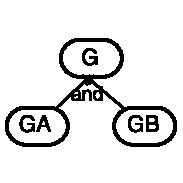
\includegraphics[scale=1]{patterns_and}} &
 \begin{lstlisting}
 Component CG {
   provides IG;
   requires
      IGA, IGB;
 }
 \end{lstlisting} \\ \hline
 Or-Refinement &
 \raisebox{-\totalheight}{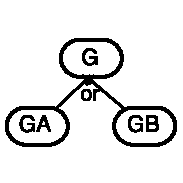
\includegraphics[scale=1]{patterns_or}} &
 \begin{lstlisting}
 Component CG {
   provides IGA;
 }
 Component CG {
   provides IGB;
 }
 \end{lstlisting} \\ \hline
 Context-condition &
 \raisebox{-\totalheight}{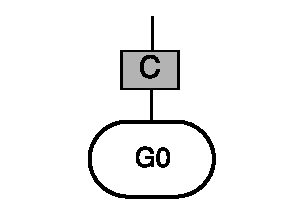
\includegraphics[scale=1]{patterns_condition}} &
 \begin{lstlisting}
 Component CG {
   provides IG;
   condition C;
 }
 \end{lstlisting} \\ \hline
\end{tabular}
\end{table}

The presented patterns for And/Or-refinements and Context-conditions, are described using goals but they can be applied for goals and plans without distinction. Both And/Or-refinements or Goal-Plans means-ends relationship will generate interfaces and components in the same way.

 pattern is applied to plans, as plans are the ones using resources, and being so they are the ones that have restrictions concerning the computing environment.

And-refinements result in components that define a strategy to achieve a given goal by achieving two or more sub, more concrete, goals.
Mapping components from an And-refinemnt results in: (i) a root interface that describe what component provides. (ii) Interfaces for each sub-goal. (iii) A component that provides the root interface and requires each interface generated for sub goals.
Such component implements a strategy to achieve its provided goal. It coordinates the sub more specific goals by calling them and passing one result as the input of another, when applicable.
As an example, applying And-refinement patterns for Root Goal - \emph{G0:Vehicle refueling is assisted} - of the Filling Station Advisor application, will result in interface IG0 and a component G0 that provides IG0 and requires IG1, IG2, IG3, IG4, and IG5.
\begin{lstlisting}
  Component G0 {
    provides IG0;
    requires IG1, IG2, IG3, IG4,IG5;
  }
\end{lstlisting}

Applying Or-refinements patterns results in a root interface definition and in multiple implementations. At the CGM, when Or-refinements are associated with context conditions, it allows for alternative strategies using different resources in the computing environment. Using the association of OR-refinement and context-conditions in the component analysis we preserve the variability present in the CGM into the architecture of the system.

For example, in the Filling Station Advisor, applying the patterns for G1:Get Position, P1:get position using GPS and P2:get position using antenna triangulation will result in the following components:

\begin{lstlisting}
  Component CP1 {
    provides IG1;
    condition C1;
  }
  Component CP2 {
    provides IG1;
    condition C2;
  }
\end{lstlisting}

The two components CP1 and CP2 provides the same goals but have different context conditions (C1:GPS and C2:antenna triangulation). It means that we can achieve the same goal using any of both resource, by deploying one of the two component variants.
That variability in the architecture allows for the adaptation to the heterogeneity in the target environment.

\subsection{Packaging}
\label{sec_artifacts}
\emph{Artifacts} are deployment units.
From the deployment point of view, the components and interfaces should be packaged in a file to be distributed. We name \emph{artifact} as such file.
An artifact should follow a standard packaging schema, so a package manager can manipulate it.
In our approach, we propose to include into the artifact metadata to describe its related goals, context conditions, and dependencies. That metadata reflects information about the packaged components. For our approach, the metadata of interest is the following:

\begin{description}
  \item[Provided goals:] goals that can be made achievable by successfully deploying the component.
  \item[Context conditions:] conditions that can be evaluated against the context. If the conditions are not satisfied it means that the component can not be deployed at the given context. This is the case when the artifact's required resources are not available in the computing environment.
  \item[Dependencies:] required goals that should be provided by other artifacts.
\end{description}

When creating the artifact we can calculate the metadata by looking at the packaged components. The artifact \emph{provided goals} metadata are the union of all \emph{provided goals} of the components packaged in an artifact. The same is valid for \emph{context conditions} and \emph{dependencies} metadata.

Both \emph{context conditions} and \emph{dependencies} impose restrictions on when an artifact can be deployed.
\emph{Context conditions} refer to the need for resources in the computing environment that are beyond the deployment agent capacity of management. Such conditions can be related to hardware implementation, e.g. presence of a GPS-module, our platform lower level software implementation, e.g. access to a protocol to query vehicle onboard computer data. If a context condition does not hold, there is nothing that can be done at deployment time to change that.
\emph{Dependencies}, on the other hand, refer to the need on other artifacts. It is specified in terms of \emph{Provided Goals}. Like other dependency management approaches, an artifact can depend on other artifacts.
Different from other approaches, we specify the dependency not to a specific version of an artifact identification but in terms of what an artifact provides.
In the Filling Station Advisor, the artifact A0, that packs the component G0 depends on IG0-definition and IG0. To satisfy the dependency, an artifacts that provides IG0-definition should be available, as well as at least one artifact that provides IG0. The Figure~\ref{fig:dependency_graph} depicts the dependency relationship between artifacts.

\begin{figure}[!htb]
  \centering
  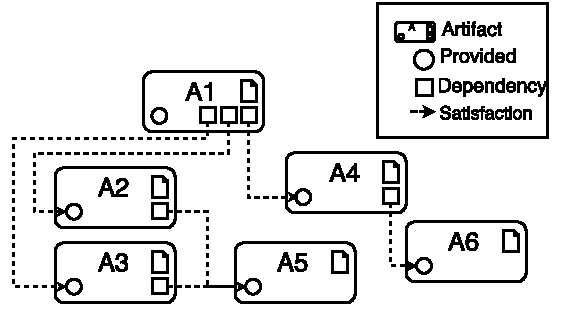
\includegraphics[width=.6\linewidth]{dependency_graph}
  \caption{Dependency Graph}
  \label{fig:dependency_graph}
\end{figure}

Artifacts are registered in a repository which allows the distribution of artifacts to the target environment. In the registration process, the artifact is uploaded to the repository, its metadata is processed, and registered in the repository database.

% Also we have a static dependency between an a component and the interfaces that describes the services it depends on.
% The interfaces and its dependencies (it being clients or implementations) can be packaged separately.
% We have an implementation dependency between a client components and any component that implements the service it depends on. That dependency can be resolved late on, in deployment time.

\subsubsection{Deployment Architectural Style}
\label{depl_arch_style}

In order to maximize the flexibility of systems following Goalp deployment approach, we propose the following architecture style to create artifacts:

Artifacts can be of 3 types:

\begin{description}
  \item[Definition] artifacts that specify the interface of goals. It contains interfaces declarations and data model. It specify the API or contracts for a given set of goals.
  The advantage of separating the goals declaration in a specific artifact is creating implementation independence.
  Goals declarations depends only on other goals declarations and have no context conditions. Goals declarations do not provide any goals.
  % Artifacts providing definitions should be unique in the repository.

  \item[Strategy] artifacts that package components that result from AND-refinements. A Goal refinement provides a high level goal and depends on other more refined goals. It should have no context condition as it do not implement plans that use specific resources in the computing environment.

  \item[Plan implementation] that artifacts contain the domain logic implementation. The plan could have dependencies on specific resources in the computing environment.
  In a dependency tree, artifacts of plan implementation type are the leaves.
  Plan implementation artifacts provides low-level goals and can have dependencies and context conditions.

\end{description}

These types of artifacts are meant to increase the flexibility of deployment.


\subsection{Development Process}

In previous subsections we see the techniques that support the design of software with variability from requirements to deployment. In this section we see how to apply this techniques in a software development process

\subsubsection{Roles}
The proposed process considers three roles: users, requirements engineers and software architects.
Figure~\ref{fig:process_roles} summarizes the collaboration between the roles.

 \begin{figure}[!htb]
   \centering
   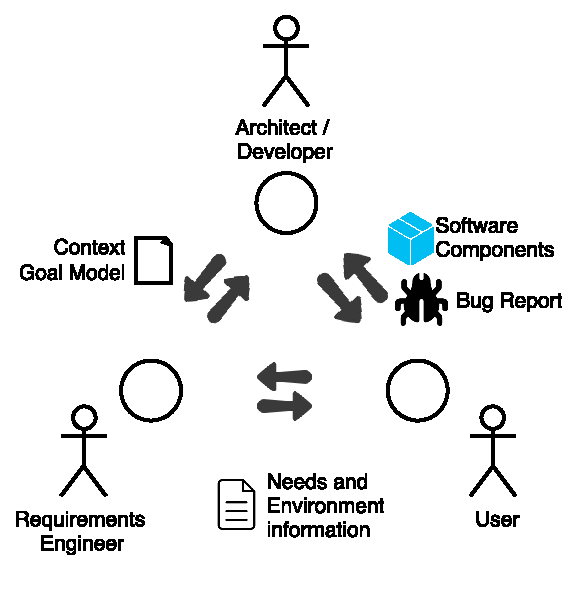
\includegraphics[width=.4\linewidth]{process_roles}
   \caption{Roles collaboration}
 \label{fig:process_roles}
 \end{figure}

\begin{description}
  \item[User]
  This role has access to a particular computing environment and wants to achieve some goals there.
  \item[Requirements Engineer]
  Is responsible for translating users goals to a contextual goal model. Also is responsible for analyzing the different contexts that the system is meant to operate and how they affect the goals.
  \item[Architect] projects the software architecture so as to permit variability of deployment.
  From the point of view of dynamic heterogeneous computing environments, the focus is to create interfaces for components that can allow for goal achievements using different computing resources.

\end{description}



\subsection{Activities}

Figure~\ref{fig:deployment_process_flow} describe the development process activities.

\label{sub:Proposal}
\begin{figure*}[!htb]
  \centering
  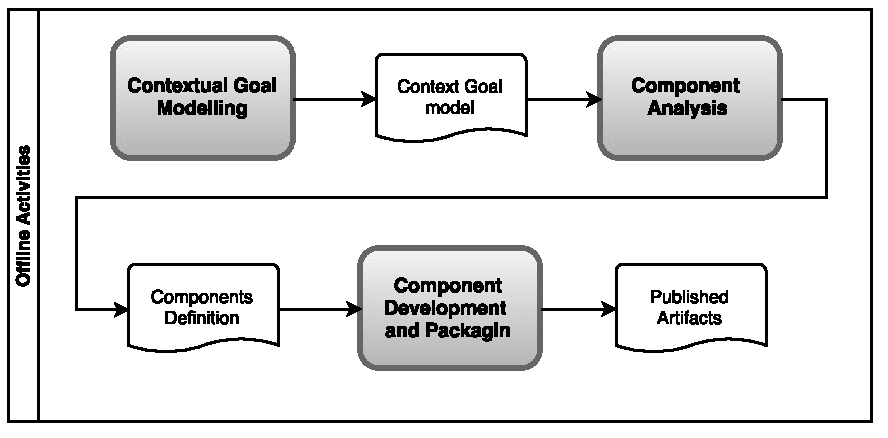
\includegraphics[width=\linewidth]{deployment_process_flow}
  \caption{Deployment Process Activities}
\label{fig:deployment_process_flow}
\end{figure*}

\subsubsection{Goal Modeling}
This phase is coordinated by a requirement engineer with the participation of a domain specialist, possibly the user.
A process such as TROPOS can be used. The output of this phase is a goal model.
The goal model has a central role in the software development process. At the goal model is identified the space of the solution, what the system should achieve, and possible strategies to achieve the goals. Also, the goal model creates a common language between users and software engineers.

\subsubsection{Context Goal Modeling}
In this activity, resources associated the domain should be identified and the Goal model should be annotated with \emph{context conditions} related to the computing environment. That analysis is a context analysis and could benefit of the process described in~\cite{ali_goal-based_2010}.

\subsubsection{Component Analysis}

Variability points are identified and componets and its interafaces are identified. Component interfaces are created following the guidelines described in Section~\ref{sec:goals_components}.

\subsubsection{Component Development}

Component development includes the cycle coding, build and test of software components.
The components are package into artifacts and should put in the repository. Artifacts are described in Section~\ref{sec_artifacts}
